\section{Business Overview}
Smoking Games started as a small video game developer. At the beginning they distributed their games through other distributers. After the great hit of a video game called ''full life'', they decided to start distributing their games on their own.\\
In 2010, after 2 years in the development business, Smoking Games became a video game developer and digital distributor company. At the start they only distributed their own games. With the growth of the enterprise, Smoking Games got many offers from other game developers to distribute their games. Smoking Games decided, that they will distribute also other developers's creations in their digital distribution section. At this point the distribution software, which is free for download for users, was named "Smoke".\\
2011 was a great year for Smoking Games: the growth of computer gaming helped consolidating the enterprise and Smoke became the distribution and gaming platform for everyone. In Smoking Games they didn't think it was enough, as their mission states: "Always creating and innovating". So they took the next step, a cloud service for saving games and cross platform gaming. Playing on two devices always moving forward in a shared game. Also, ''full life 3'' was released during this year, giving Smoking Games a very good position in the market as a trusted game developer.\\
In 2012, after 4 years in a rented placement, the headquarter of Smoking Games moved to a newly owned location. Taking advantage of this growth the whole enterprise grew. It redefined in this year still at the same size of 35 employees fixed plus some external services. Even though the enterprise organization is quite horizontal, the shares and benefits belong to the employees and bosses in the same amount, they keep a minimal organization for political purposes. The hierarchy of the enterprise is shown in figure \ref{fig:org_hierarchy}.

\begin{figure}[htpb]\centering
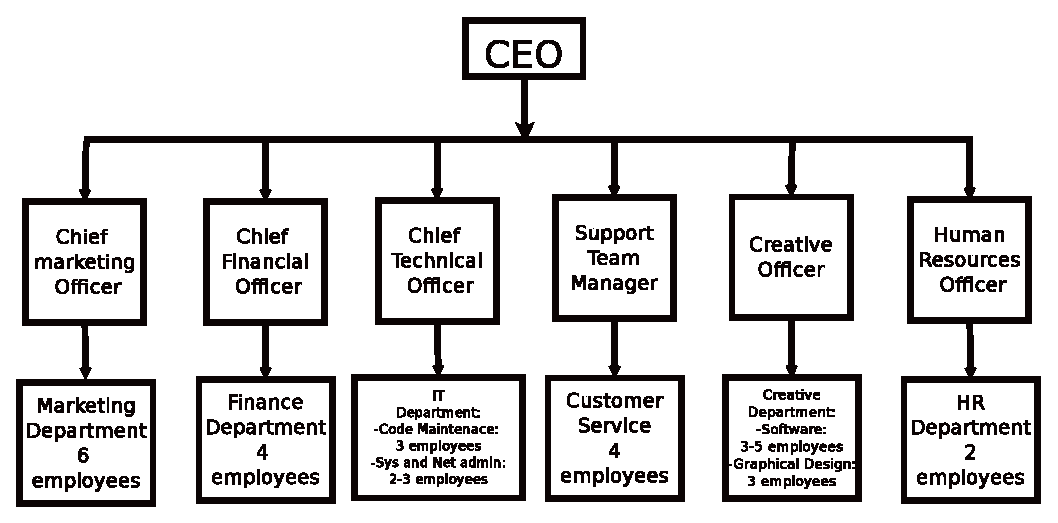
\includegraphics[ width={0.7\textwidth} ] {pictures/Organizational_hierarchy}
\caption{Organizational hierarchy}
\label{fig:org_hierarchy}
\end{figure}
\newpage
\noindent The main source of income for Smoking Games is selling their own games. These sales give a 100\% of the price back. The games produced by other companies are a different story: for every game and developer Smoking Games makes a different contract, going from the 75 to the 50\% money of the sales in the distribution price.\\
Smoking Games is located in a building in Tenerife, Spain. The building next to it is one of the main hubs for telefonica SA, main internet company in Spain. Like this the internet conection is much more ensured. This is important because most of Smoking Games's business is done over the internet.
